% Options for packages loaded elsewhere
\PassOptionsToPackage{unicode}{hyperref}
\PassOptionsToPackage{hyphens}{url}
%
\documentclass[ignorenonframetext,aspectratio=169]{beamer}

\usepackage{pgfpages}

\setbeamertemplate{caption}[numbered]
\setbeamertemplate{caption label separator}{: }
\setbeamercolor{caption name}{fg=normal text.fg}
\beamertemplatenavigationsymbolsempty

% Prevent slide breaks in the middle of a paragraph
\widowpenalties 1 10000
\raggedbottom
\setbeamertemplate{part page}{
  \centering
  \begin{beamercolorbox}[sep=16pt,center]{part title}
    \usebeamerfont{part title}\insertpart\par
  \end{beamercolorbox}
}
\setbeamertemplate{section page}{
  \centering
  \begin{beamercolorbox}[sep=12pt,center]{part title}
    \usebeamerfont{section title}\insertsection\par
  \end{beamercolorbox}
}
\setbeamertemplate{subsection page}{
  \centering
  \begin{beamercolorbox}[sep=8pt,center]{part title}
    \usebeamerfont{subsection title}\insertsubsection\par
  \end{beamercolorbox}
}
\AtBeginPart{
  \frame{\partpage}
}
\AtBeginSection{
  \ifbibliography
  \else
    \frame{\sectionpage}
  \fi
}
\AtBeginSubsection{
  \frame{\subsectionpage}
}

\usepackage{amsmath,amssymb}
\usepackage{iftex}
\ifPDFTeX
  \usepackage[T1]{fontenc}
  \usepackage[utf8]{inputenc}
  \usepackage{textcomp} % provide euro and other symbols
\else % if luatex or xetex
  \usepackage{unicode-math}
  \defaultfontfeatures{Scale=MatchLowercase}
  \defaultfontfeatures[\rmfamily]{Ligatures=TeX,Scale=1}
\fi

\usepackage{lmodern}
\ifPDFTeX\else  
    % xetex/luatex font selection
\fi

% Use upquote if available, for straight quotes in verbatim environments
\IfFileExists{upquote.sty}{\usepackage{upquote}}{}
\IfFileExists{microtype.sty}{% use microtype if available
  \usepackage[]{microtype}
  \UseMicrotypeSet[protrusion]{basicmath} % disable protrusion for tt fonts
}{}
\makeatletter
\@ifundefined{KOMAClassName}{% if non-KOMA class
  \IfFileExists{parskip.sty}{%
    \usepackage{parskip}
  }{% else
    \setlength{\parindent}{0pt}
    \setlength{\parskip}{6pt plus 2pt minus 1pt}}
}{% if KOMA class
  \KOMAoptions{parskip=half}}
\makeatother
\usepackage{xcolor}
\newif\ifbibliography
\setlength{\emergencystretch}{3em} % prevent overfull lines
\setcounter{secnumdepth}{-\maxdimen} % remove section numbering


\providecommand{\tightlist}{%
  \setlength{\itemsep}{0pt}\setlength{\parskip}{0pt}}\usepackage{longtable,booktabs,array}
\usepackage{calc} % for calculating minipage widths
\usepackage{caption}
% Make caption package work with longtable
\makeatletter
\def\fnum@table{\tablename~\thetable}
\makeatother
\usepackage{graphicx}
\makeatletter
\def\maxwidth{\ifdim\Gin@nat@width>\linewidth\linewidth\else\Gin@nat@width\fi}
\def\maxheight{\ifdim\Gin@nat@height>\textheight\textheight\else\Gin@nat@height\fi}
\makeatother
% Scale images if necessary, so that they will not overflow the page
% margins by default, and it is still possible to overwrite the defaults
% using explicit options in \includegraphics[width, height, ...]{}
\setkeys{Gin}{width=\maxwidth,height=\maxheight,keepaspectratio}
% Set default figure placement to htbp
\makeatletter
\def\fps@figure{htbp}
\makeatother

\makeatletter
\makeatother
\makeatletter
\makeatother
\makeatletter
\@ifpackageloaded{caption}{}{\usepackage{caption}}
\AtBeginDocument{%
\ifdefined\contentsname
  \renewcommand*\contentsname{Daftar Isi}
\else
  \newcommand\contentsname{Daftar Isi}
\fi
\ifdefined\listfigurename
  \renewcommand*\listfigurename{Daftar Gambar}
\else
  \newcommand\listfigurename{Daftar Gambar}
\fi
\ifdefined\listtablename
  \renewcommand*\listtablename{Daftar Tabel}
\else
  \newcommand\listtablename{Daftar Tabel}
\fi
\ifdefined\figurename
  \renewcommand*\figurename{Gambar}
\else
  \newcommand\figurename{Gambar}
\fi
\ifdefined\tablename
  \renewcommand*\tablename{Tabel}
\else
  \newcommand\tablename{Tabel}
\fi
}
\@ifpackageloaded{float}{}{\usepackage{float}}
\floatstyle{ruled}
\@ifundefined{c@chapter}{\newfloat{codelisting}{h}{lop}}{\newfloat{codelisting}{h}{lop}[chapter]}
\floatname{codelisting}{Daftar}
\newcommand*\listoflistings{\listof{codelisting}{Daftar Daftar}}
\makeatother
\makeatletter
\@ifpackageloaded{caption}{}{\usepackage{caption}}
\@ifpackageloaded{subcaption}{}{\usepackage{subcaption}}
\makeatother
\makeatletter
\@ifpackageloaded{tcolorbox}{}{\usepackage[skins,breakable]{tcolorbox}}
\makeatother
\makeatletter
\@ifundefined{shadecolor}{\definecolor{shadecolor}{rgb}{.97, .97, .97}}
\makeatother
\makeatletter
\makeatother
\makeatletter
\makeatother

\ifLuaTeX
\usepackage[bidi=basic]{babel}
\else
\usepackage[bidi=default]{babel}
\fi
\babelprovide[main,import]{indonesian}

% get rid of language-specific shorthands (see #6817):
\let\LanguageShortHands\languageshorthands
\def\languageshorthands#1{}

\ifLuaTeX
  \usepackage{selnolig}  % disable illegal ligatures
\fi

\IfFileExists{bookmark.sty}{\usepackage{bookmark}}{\usepackage{hyperref}}
\IfFileExists{xurl.sty}{\usepackage{xurl}}{} % add URL line breaks if available
\urlstyle{same} % disable monospaced font for URLs

\usepackage{minted}

\newminted{julia}{breaklines,fontsize=\footnotesize}
\newminted{python}{breaklines,fontsize=\footnotesize}

\newminted{bash}{breaklines,fontsize=\footnotesize}
\newminted{text}{breaklines,fontsize=\footnotesize}

\newcommand{\txtinline}[1]{\mintinline[breaklines,fontsize=\footnotesize]{text}{#1}}
\newcommand{\jlinline}[1]{\mintinline[breaklines,fontsize=\footnotesize]{julia}{#1}}
\newcommand{\pyinline}[1]{\mintinline[breaklines,fontsize=\footnotesize]{python}{#1}}



\title{TF2202 Komputasi Rekayasa\\
Aproksimasi, Kesalahan Pemotongan dan Pembulatan}
\author{Fadjar Fathurrahman}
\date{2024}

\begin{document}

\frame{\titlepage}

\begin{frame}{Kesalahan numerik (\textit{numerical errors})}

kesalahan (galat) pemotongan (truncation error)

kesalahan (galat) pembulatan (round-off error)

\begin{equation*}
\text{nilai benar} = \text{aproksimasi} + \text{galat}
\end{equation*}

\begin{equation*}
E_{t} = \text{nilai benar} - \text{aproksimasi}
\end{equation*}
$E_t$: galat sebenarnya

\end{frame}


\begin{frame}{Galat relatif sebenarnya}

Definisi galat sebenarnya tidak memperhitungkan orde atau besar
dari nilai yang sedang dibahas: manakah yang memiliki galat lebih
besar?:
\begin{itemize}\tightlist
\item galat 1 cm dari pengukuran panjang meja
\item galat 1 cm dari pengukuran panjang jembatan atau jalan raya
\end{itemize}

Alternatif yang dapat digunakan
adalah menggunakan \textit{galat relatif}:
\begin{equation*}
\text{galat relatif sebenarnya} = \frac{\text{galat sebenarnya}}{\text{nilai benar}}
\end{equation*}
atau dinyatakan dalam persentase
\begin{equation*}
\epsilon_{t} = \frac{\text{galat sebenarnya}}{\text{nilai benar}} \times 100\%
\end{equation*}

\end{frame}



\begin{frame}{Galat aproksimasi}

Pada kondisi riil, nilai sebenarnya biasanya tidak diketahui \textit{a priori}.
Dalam kondisi ini, kita dapat menggunakan galat aproksimasi:
\begin{equation*}
\epsilon_{a} = \frac{\text{galat aproksimasi}}{\text{aproksimasi}}
\end{equation*}

Dalam aplikasinya juga dapat digunakan definisi lain dari galat aproksimasi.
Misalnya pada kasus pendekatan \textit{iteratif} di mana aproksimasi dilakukan
berulang, nilai aproksimasi dihitung berdasarkan nilai aproksimasi sebelumnya.
Pada kasus ini kita dapat menggunakan:
\begin{equation*}
\epsilon_{a} = \frac{\text{aproksimasi sekarang} - \text{aproksimasi sebelumnya}}%
{\text{aproksimasi sekarang}} \times 100\%
\end{equation*}
Proses iteratif biasanya diulangi sampai nilai $\epsilon_{a}$ mencapai atau
lebih kecil dari nilai tertentu, misalnya $\epsilon_{s}$:
\begin{equation*}
\left| \epsilon_{a} \right| < \epsilon_{s}
\end{equation*}


\end{frame}


\begin{frame}{Kriteria Scarborough}

Scarborough mengusulkan suatu kriteria berikut:
\begin{equation*}
\epsilon_{s} = (0.5 \times 10^{2-n})\%
\end{equation*}
yang mana jika kriteria ini terpenuhi maka hasil numerik yang kita peroleh
benar sedikitnya dalam $n$ angka penting (\textit{significant figures}).

\end{frame}



\begin{frame}[fragile]{Contoh: deret Maclaurin}
\fontsize{9}{10}\selectfont

Tinjau deret Maclaurin berikut:
\begin{equation*}
e^{x} = 1 + x + \frac{x^2}{2!} + \frac{x^3}{3!} + \cdots + \frac{x^{n}}{n!}
\end{equation*}
Misalnya kita ingin menentukan nilai dari $e^{0.5}$ menggunakan deret Maclaurin ini.
Kita ingin agar hasil aproksimasi yang kita peroleh benar setidaknya 3 angka penting.
Menggunakan kriteria Scarborough kita dapat menghitung $\epsilon_s$ yang
diperlukan (dengan $n=3$):
\begin{equation*}
\epsilon_{s} = (0.5 \times 10^{2-3})\% = 0.05\% = 0.0005
\end{equation*}

Pertama, kita dapat menggunakan hanya dua suku:
$$
e^{x} = 1 + x
$$
dengan $x = 0.5$ diperoleh:
$$
e^{0.5} = 1 + 0.5 = 1.5
$$
Karena $e^{0.5}$ dapat dihitung dengan menggunakan pustaka atau fungsi \pyinline{exp}
pada Python, kita dapat menghitung galat sebenarnya dengan menganggap bahwa keluaran
dari fungsi \pyinline{exp} adalah nilai sebenarnya:
$$
\epsilon_{t} = \frac{1.648721 - 1.5}{1.648721} \times 100\% = 9.02\%
$$
\end{frame}


\begin{frame}[fragile]{Contoh: deret Maclaurin}
\fontsize{9}{10}\selectfont

\end{frame}



\begin{frame}{Kesalahan Pemotongan (\textit{Round-off Error})}

Galat pembulatan berhubungan langsung dengan bagaimana cara suatu bilangan
disimpan pada komputer.

Sistem bilangan: suatu konvensi untuk merepresentasikan
kuantitas numerik.
Untuk manusia, yang paling natural digunakan adalah sistem desimal atau
basis-10. Pada sistem ini ada 10 digit: 0-9. Setiap digit memiliki nilai tempat.
Contoh:
$$
86409 = (8 \times 10^4) + (6 \times 10^3) + (4 \times 10^2) + (0 \times 10^1) +
(9\times 10^0)
$$

Komputer menggunakan basis-2 untuk merepresentasikan bilangan atau sistem biner.
Pada sistem ini hanya ada dua digit: 0 dan 1.
Contohnya bilangan biner $101.1_{2}$ sama dengan:
\begin{equation*}
1 \times 2^2 + 0 \times 2^1 + 1 \times 2^0 + 1 \times 2^{-1} = 4 + 0 + 1 + 0.5 = 5.5_{10}
\end{equation*}
Biasanya notasi basis pada $5.5_{10}$ tidak ditampilkan, hanya ditulis $5.5$.

\end{frame}



\begin{frame}

{\centering
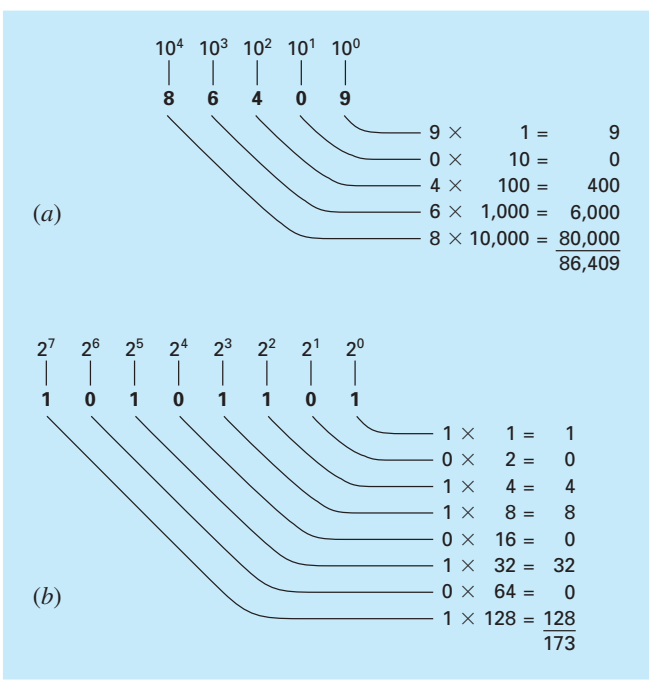
\includegraphics[height=0.8\textheight]{../chapra_7th/Chapra_Fig_3_5.png}
\par}

\end{frame}


\begin{frame}{Representasi bilangan bulat (integer)}

Metode magnitudo bertanda, \textit{signed magnitude method}, digunakan pada komputer
untuk merepresentasikan suatu bilangan. Bit pertama digunakan untuk menyatakan tanda
(0 untuk bilangan positif dan 1 untuk bilangan negatif).
Bit yang lain digunakan untuk menyimpan magnitudo bilangan.
Misalnya bilangan -173 pada komputer dengan 16-bit

{\centering
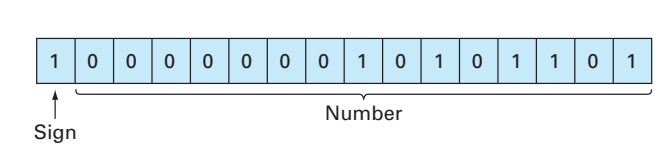
\includegraphics[height=0.3\textheight]{../chapra_7th/Chapra_Fig_3_6.png}
\par}

\end{frame}


\begin{frame}{Contoh representasi bilangan bulat}

Tentukan bilangan bulat dalam basis-10 yang dapat direpresentasikan dalam 16-bit.

Dari 16 bit yang tersedia, bit pertama digunakan menyimpan tanda.
15 bit yang tersisa dapat digunakan untuk menyimpan bilangan biner
dari 0 sampai 111111111111111 yang sama dengan
$$
(1 \times 2^{14}) + (1 \times 2^{13}) + \cdots +
(1 \times 2^{1}) + (1 \times 2^{0}) = 32767
$$
Oleh karena itu 16 bit dapat digunakan untuk merepresentasikan bilangan bulat
dari -32767 sampai 32767
Bilangan 0 sudah didefinisikan sebagai 0000000000000000, maka
1000000000000000 tidak perlu digunakan untuk menyatakan minus 0. Oleh karena itu
biasanya representasi biner tersebut digunakan untuk mereprentasikan bilangan
negatif tambahan, yaitu -32768.

\end{frame}



\begin{frame}[fragile]{Metode komplemen-2}

Pada komputer modern, metode magnitudo bertanda yang dijelaskan sebelumnya
tidak secara langsung digunakan. Metode alternatif (namun masih terkait)
yaitu metode komplemen-2 (\textit{2's complement}) digunakan. Pada metode ini
kita tidak memerlukan bit khusus untuk menyimpan tanda.

Misalnya kita ingin menyatakan bilangan -28 pada komputer 8-bit.
Pertama angka 28 dinyatakan dalam bilangan biner, yaitu:
\begin{textcode}
00011100
\end{textcode}
Untuk menyatakan angka -28, pertama kita inversi bilangan biner tersebut
(0 menjadi 1, 1 menjadi 0):
\begin{textcode}
11100011
\end{textcode}
kemudian tambahkan 1:
\begin{textcode}
11100100
\end{textcode}

\end{frame}


\begin{frame}{\textit{Overflow} dan \textit{underflow}}

Detil mengenai representasi bilangan pada komputer tidak menjadi fokus dalam
kuliah ini, namun pesan yang ingin disampaikan adalah \textbf{adanya
limitasi jika kita merepresentasi bilangan bulat pada komputer dengan
jumlah bit yang terbatas}.

Tipe bilangan bulat yang sering digunakan adalah \texttt{Int32} (menggunakan
32 bit) dan \texttt{Int64} (menggunakan 64 bit). Beberapa bahasa pemrograman juga
mendukung \texttt{Int16} dan \texttt{Int8}.
Untuk tiap tipe bilangan bulat atau integer tersebut, ada nilai terbesar
dan terkecil yang dapat direpresentasikan.

Jika operasi perhitungan yang kita lakukan menghasilkan
bilangan bulat yang lebih besar dari rentang nilai yang mungkin
maka yang terjadi adalah \textit{overflow}

Jika operasi perhitungan yang kita lakukan menghasilkan
bilangan bulat yang lebih kecil dari rentang nilai yang mungkin
maka yang terjadi adalah \textit{underflow}

\end{frame}




\begin{frame}[fragile]{Catatan khusus untuk Python}

Pada Python kita tidak perlu mendeklarasikan terlebih dahulu suatu variabel memiliki
suatu tipe tertentu. Tipe suatu variabel pada Python dapat berubah-ubah (dinamis), dan
biasanya secara \textit{default} dapat terjadi konversi tipe secara \textit{implisit} (otomatis, tidak
perlu diperintahkan oleh \textit{programmer} atau pengguna).

Sebagai demonstrasi, coba perhatikan keluaran dari kode ini:
\begin{pythoncode}
a = 2
type(a) # int
# Ubah variabel a
a = a + 1.1
type(a) # float
\end{pythoncode}

\end{frame}



\begin{frame}[fragile]{Catatan khusus untuk Python}

Tipe data integer \textit{default} pada Python bukanlah tipe integer yang umum.
\pyinline{int} pada Python merupakan tipe bilangan bulat khusus yang dirancang agar dapat
memiliki lebar bit yang adaptif, sehingga tidak memungkinkan terjadinya
\textit{overflow} maupun \textit{underflow}.

Tipe data \texttt{Int32} dan \texttt{Int64} (dan juga beberapa tipe data dengan lebar bit
tetap) dapat kita akses melalui pustaka Numpy. Pada pustaka Numpy, tipe-tipe data
tersebut dapat diakses dengan menggunakan \pyinline{np.int32} dan \pyinline{np.int64}.
Numpy juga menyediakan tipe data \pyinline{np.int8} dan \pyinline{np.int16}.
Fungsi \pyinline{np.iinfo()} dapat digunakan untuk mengetahui nilai terbesar
dan terkecil yang mungkin untuk setiap tipe data tersebut.

\begin{pythoncode}
import numpy as np
np.iinfo(np.int16)
\end{pythoncode}

\end{frame}




\begin{frame}[fragile]{Contoh Python}

Fungsi \pyinline{type} dapat digunakan untuk mengetahui tipe dari suatu
variabel.

\begin{pythoncode}
import numpy as np
a = np.int8(127) # variabel a dengan tipe np.int8
b = np.int8(a + 1) # berapa nilai b? Seharusnya ini akan menghasilkan overflow
type(a), type(b)
# TUGAS: Coba lakukan operasi yang menghasilkan underflow
\end{pythoncode}

Pada kode berikut ini Python akan melakukan konversi ke tipe dengan lebar bit
yang lebih besar.
\begin{pythoncode}
a = np.int(127)
b = a + 1
type(a), type(b) # sekarang apakah tipe dari b?
\end{pythoncode}

\end{frame}


\begin{frame}{Representasi bilangan titik-mengambang (\textit{floating point})}

Kuantitas numerik dengan pecahan dan yang memiliki digit di belakang koma, biasanya direpresentasikan
pada komputer dengan menggunakan format bilangan titik-mengambang atau sering disebut sebagai
\textit{floating-point number}. Pada pendekatan ini, suatu bilangan dinyatakan sebagai:
\begin{equation*}
\pm s \times b^{e}
\end{equation*}
dengan $s$ adalah significand atau mantissa, $b$ adalah basis dari sistem
bilangan yang digunakan, dan $e$ adalah eksponen.
  
Sebelum dinyatakan dalam bentuk ini, suatu bilangan dinormalisasi terlebih dahulu dengan cara
memindahkan titik, desimal, biner dan sebagainya sedemikian rupa sehingga hanya satu digit
yang berada di kiri tanda titik. Hal ini dilakukan untuk menghemat memori karena tidak ada
bilangan nol yang tidak signifikan yang perlu disimpan.

Misalnya bilangan 0.005678 dapat direpresentasikan tanpa normalisasi sebagai
$0.005678 \times 10^{0}$. Namun dengan normalisasi, nilai tersebut akan disimpan
sebagai $5.678 \times 10^{-3}$, artinya dua nol sebelum digit 5 tidak perlu disimpan.

Ketika kita melakukan normalisasi untuk bilangan dengan basis 2, digit yang berada di kiri tanda
titik biner akan selalu bernilai 1.

\end{frame}


% URL: https://0.30000000000000004.com/
% https://discourse.julialang.org/t/incorrect-summation-of-float64/93376


\end{document}
